\documentclass{article}

\usepackage{geometry}
\geometry{letterpaper, total={7in, 10in} }

\usepackage{listings}
\usepackage{hyperref}
\usepackage{booktabs}
\usepackage{graphicx}
\usepackage{verbatim}
\usepackage{appendix}
\usepackage{url}
\lstset{breaklines=True}
\graphicspath{./Figures/}
\title{Evaluating Graph Sampling Methods for Graph Attention Networks on Citation Networks}
\author{Ayush Kumar, Nick Puglisi}
\date{December 17, 2021}

\begin{document}
	\maketitle
	\tableofcontents
	\pagebreak
	\section{Introduction}
	
	Graph Convolutional Network (GCNs) have been a great contribution to the field of network data ever since Thomas Kipf and Max Welling published the paper: Semi-Supervised Classification With Graph Convolutional Networks \cite{kipf2017semisupervised}. The main idea behind the paper is that since graph structures do not exhibit euclidean geometry, standard convolutions that might be used for image recognition will not translate onto graph structures as well. So, through the use of Laplacian re-normalization trick presented in the GCN paper, classification accuracy	has increased in comparison to other similar methods. However, a major tenet in the field of machine learning is that there is no one best method to employ for each and every problem. So, we present an investigation into both sampling techniques combined with Graphical Attention Networks (GATs).

	\subsection{Motivation}
	
	What sparked the investigation presented here was an observation made from the methodology  in the original GCNs paper. 
	Throughout model training, Kipf and Welling employed random dropout of nodes to introduce stochasticity during gradient descent. However, the use of random dropout only allows
	for updates to occur once per epoch while requiring the full data set to be loaded for every training iteration. So, some questions arose on if 
	sampling methods could be employed over random dropout to increase efficiency when combined with the Graphical Attention Networks
	
	\subsection{Overview of Graph Attention Networks}
	
	One shortcoming of the GCNs methodology is that it assumes equal importance of neighboring nodes. While some network structures might allow for
	an assumption like this to be made, other network structures might not allow for this assumption. So in the paper, 
	Graphical Attention Networks \cite{velockovic2018graph}, the authors seek to address this by leveraging self-attentional layers to enable different weights to be assigned across a given cluster of nodes. 
	The GATs method also used dropout to introduce stochasticity and pushed results that successfully achieved or beat other methods of node classification, all while 
	removing the need for equal importance.

	\subsection{Overview of Graph Sampling Methods} 
	
	Both GCNs and GATs methodology employed the use of dropout during model training. However, as the size of a network increases,
	it becomes much more computationally expensive to train a model, for full-batch training only allows for parameters to update once per epoch. This sharp increase in power needed for model training has thus created a need for a way to minimize both storage costs and time spent.
	In the paper Sampling Methods for Efficient Training of Graph Convolutional Networks: A Survey \cite{liu2021sampling}, the authors survey and outline a whole host 
	of sampling methods along with their respective algorithms that promise an increases in training efficiency. The methods outlined fall into two categories, namely: Layer-wise and subgraph-based sampling. One of the downsides of using sampling methods
	is that a bias-variance trade-off will be introduced. Yet, motivated by both GATs and the sampling methods applied to GCNs, we ask: is there any gain to applying sampling to the Graphical Attention Networks?
	
	We will begin by selecting three different sampling methods to apply to the GATs, namely: GraphSAGE, GraphSAINT, and ClusterGCN. The first, GraphSAGE, trains the model through an inductive process in which neighborhood sampling is undertaken. That is, sampling is carried out by 
	selecting neighboring nodes for each node in the graph followed by aggregation. This greatly reduces the computational costs since only the sampled nodes need be loaded. The Figure below outlines the algorithm for GraphSAGE:
	\begin{center}
		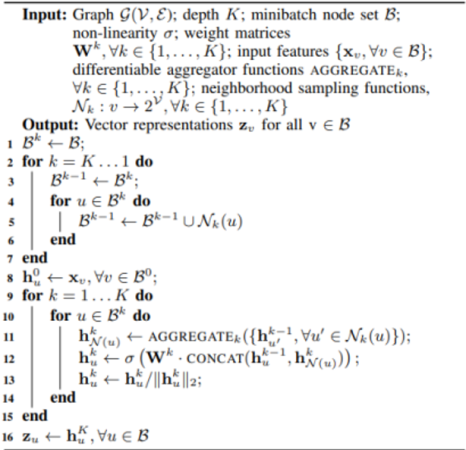
\includegraphics[scale=0.4]{Figures/sage.png} 
	\end{center}
	
	The next sampling method selected for application is GraphSAINT \cite{graphsaint-iclr20}. GraphSAINT deploys a sampler used to estimate the probability of nodes and edges being sampled. Now, in each batch, subgraphs deemed to be appropriate according to the sampler are selected and a full GCN is then built and trained.
	The figure below outlines the sampling algorithm eployed by GraphSAINT:
	
	\begin{center}
		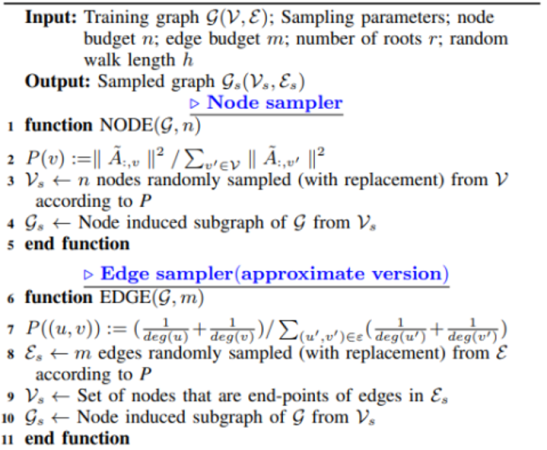
\includegraphics[scale=0.4]{Figures/saint1.png}
		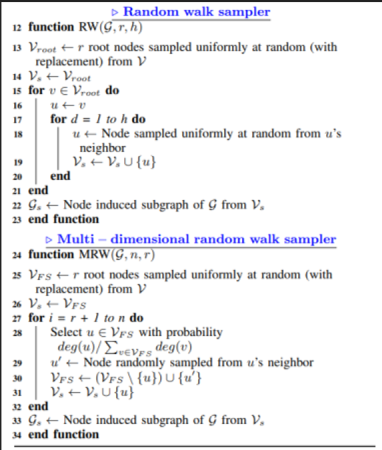
\includegraphics[scale=0.4]{Figures/saint2.png}
	\end{center}
	
	
	The final sampling method employed for this analysis is ClusterGCN \cite{2019}. As the name of the method suggests, ClusterGCN employs the use of sampling onto subgraphs and clusters. A given graph is first partitioned into multiple clusters that then get randomly sampled as a batch to form a subgraph. Finally, each iteration of training is carried out on a subgraph previously generated. Since only a subgraph needs to be loaded for each training iteration, the overall memory requirement scales well!
	The figure below outlines the training algorithm employed by the ClusterGCN sampling method:
	
	\begin{center}
		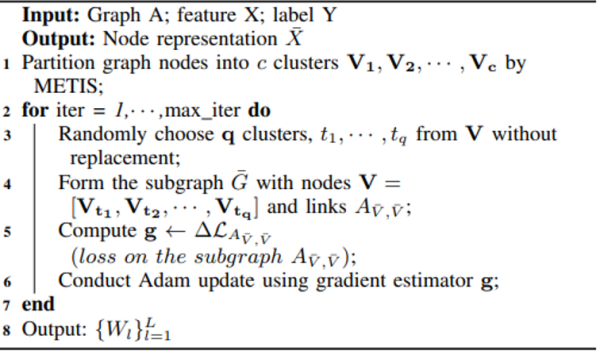
\includegraphics[scale=0.6]{Figures/cluster.png}
	\end{center}

	
	\section{Testing and Evaluation}
	
	\subsection{Testing Setup}
	
	The sampling methods were tested on three citation networks originally featured in the original Graph Attention Networks paper: Cora, Citeseer, and PubMed. The following table summarizes the key characteristics of the datasets. 
	
	\begin{center}
		\begin{tabular}{|l|c|c|c|}
			\hline
			& Cora & Citeseer & PubMed \\ \hline
			\# Nodes            & 2708 & 3327     & 19717  \\ \hline
			\# Edges            & 5429 & 4732     & 44338  \\ \hline
			\# Features         & 1433 & 3703     & 500    \\ \hline
			\# Classes          & 7    & 6        & 3      \\ \hline
			\# Training Nodes   & 140  & 120      & 60     \\ \hline
			\# Validation Nodes & 500  & 500      & 500    \\ \hline
			\# Test Nodes       & 1000 & 1000     & 1000   \\ \hline
		\end{tabular}
	\end{center}
	
	The same architecture was used for all the datasets, and they were tested using the following sampling methods described in the literature review: Random Node Sampler, ClusterGCN, GraphSAGE Mini-Batch Sampling, GraphSAINT Node Sampling, GraphSAINT Edge Sampling, GraphSAINT Random Walk Sampling. 


	\subsection{Results}
	
	Below are the results of the sampling methods, based on average testing accuracy over four trials. Comparable results have been bolded. 
	

	\begin{center}

		\begin{tabular}{c|l|l|l|}
			\cline{2-4}
			& \multicolumn{1}{c|}{Cora} & \multicolumn{1}{c|}{CiteSeer} & PubMed          \\ \hline
			\multicolumn{1}{|c|}{Baseline (No Sampling)}         & \textbf{82.0\%}           & \textbf{69.9\%}               & \textbf{77.0\%} \\ \hline
			\multicolumn{1}{|c|}{Random Node Sampler}            & 77.6\%                    & 65.2\%                        & 73.4\%          \\ \hline
			\multicolumn{1}{|c|}{ClusterGCN}                     & \textbf{80.8\%}           & \textbf{70.7\%}               & \textbf{77.1\%} \\ \hline
			\multicolumn{1}{|c|}{GraphSAGE}                      & 59.3\%                    & \textbf{70.9\%}               & \textbf{76.3\%} \\ \hline
			\multicolumn{1}{|c|}{GraphSAINT Node Sampler}        & 60.9\%                    & 34.2\%                        & 26.4\%          \\ \hline
			\multicolumn{1}{|c|}{GraphSAINT Edge Sampler}        & 70.7\%                    & 50.5\%                        & 55.7\%          \\ \hline
			\multicolumn{1}{|c|}{GraphSAINT Random Walk Sampler} & \textbf{79.9\%}           & 68.6\%                        & 75.3\%          \\ \hline
		\end{tabular}
	
	\end{center}

	\section{Conclusion}
	
	Based on experimental results we observe that sampling methods can be effectively utilized to match or even surpass performance of baseline models. We also observe that while some sampling methods are all around excellent like ClusterGCN, others performance varies greatly with the dataset, like GraphSAGE or the GraphSAINT Random Walk Sampler. Since Graph Attention Networks depend on embedding based on neighbors it is not surprising that subgraph based methods that preserve neighborhood outperformed stochastic edge or node-based methods. There is no singular best sampling method in any case, and the best method may vary by dataset size and structure. There is no free lunch when it comes to sampling for Graph Attention Networks. 
	
	Effective sampling for GATs opens the door for future research in efficient computation on much larger datasets without exploding training times, and allowing for multiple gradient updates every epoch. Matching the performance of the baseline method is a massive victory for computational efficiency. Baseline methods were trained for 1000 epochs while the sampling methods were only trained for 100 epochs, and many converged even sooner. 
	
	\nocite{*}
	\pagebreak
	\bibliographystyle{plain}
	\bibliography{refs}
	

	\pagebreak
	\appendix
	\section{Code}
	This is the code used to run the Cora sampling procedures. Other datasets were used by simply changing the dataset name in the initial definition. For this reason, only the Cora sampling script is included in this document. 
	
	\lstinputlisting[language=python]{../python/cora_sampling.py}

	
\end{document}